\subsection{Applying the forward-backward procedure}

\begin{frame} 
\mode<presentation>{
    \begin{center} \huge
        \subsecname
    \end{center}
    
    

\begin{equation}
P(\vec m^{(t)} | \{\vec x^{(s)}\}_{s=1}^T )
\;=\;
\frac{
{\color{orange}
P( \vec x^{(t+1)}, \ldots, \vec x^{(T)} | \vec m^{(t)} )
}
\cdot 
{\color{blue}
P(\vec m^{(t)}, \vec x^{(1)}, \ldots, \vec x^{(t)}) 
}
}{
P(\vec x^{(1)}, \ldots, \vec x^{(T)})
}
\end{equation}
    }
\end{frame}

\subsubsection{Inference}

\begin{frame}{\subsecname:~\subsubsecname}

Inference using the conditional distribution
$
P(\vec m^{(t)} | \{\vec x^{(s)}\}_{s=1}^T )
$

Example: ``Change detection''

\begin{equation}
P(\vec m^{(t)} \ne \vec m^{(t-1)} | \{\vec x^{(s)}\}_{s=1}^T )
\end{equation}

\svspace{5mm}

\slidesonly{
\begin{center}
	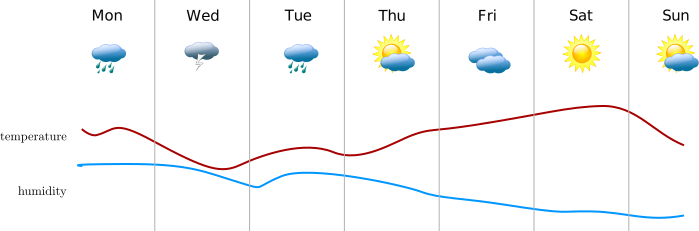
\includegraphics[width=0.6\textwidth]{img/weather}
	\captionof*{figure}{What are the chances of two sunny days in a row?}
\end{center}
}

\end{frame}

\subsubsection{Parameter estimation}

\begin{frame}{\subsecname:~\subsubsecname}

Estimate the parameters $\vec{w} := \{
		\vec{A},
		\vec{b},
		\vec{\boldsymbol{\phi}}
		\}$ of an HMM.\\
		
The forward-backward procedure needs the parameters to be known but they need not necessarily be optimal.

\pause

\slidesonly{
\begin{center}
	
\includegraphics[width=0.3\textwidth]{img/meme_fwdbwdwork}
\end{center}
}

\end{frame}

\begin{frame}{\subsecname:~\subsubsecname}

\question{How do we estimate the parameters of an HMM?}

\pause

-Combine the forward-backward procedure with Expectation Maximization

\slidesonly{
\begin{center}
	
\includegraphics[width=0.5\textwidth]{img/meme_fwdbwdemintro}
\end{center}
}

\end{frame}

\begin{frame}{\subsubsecname}

\begin{block}{Baum-Welch Algorithm}
\begin{enumerate}
\item The forward-backward procedure is given intermediate estimates of the parameters to compute the distributions
\item The EM algorithm updates the parameters to maximize the likelihood of the data.
\end{enumerate}
\end{block}

\end{frame}

\subsubsection{Sampling from the posterior}

\begin{frame}{Only}
\frametitle{\subsecname:~\subsubsecname}

The forward-backward procedure can be applied to sample from the posterior
$
P(\{\vec m^{(t)} \} | \{\vec x^{(t)}\} )
$

\begin{itemize}
\item<only@1>
Example from speech recognition where
\begin{itemize}
\item $\{\vec m^{(t)} \}$ represents the sequence of phonemes,
\item $\{\vec x^{(t)} \}$ samples from audio file with speech.
\end{itemize}

\begin{center}
	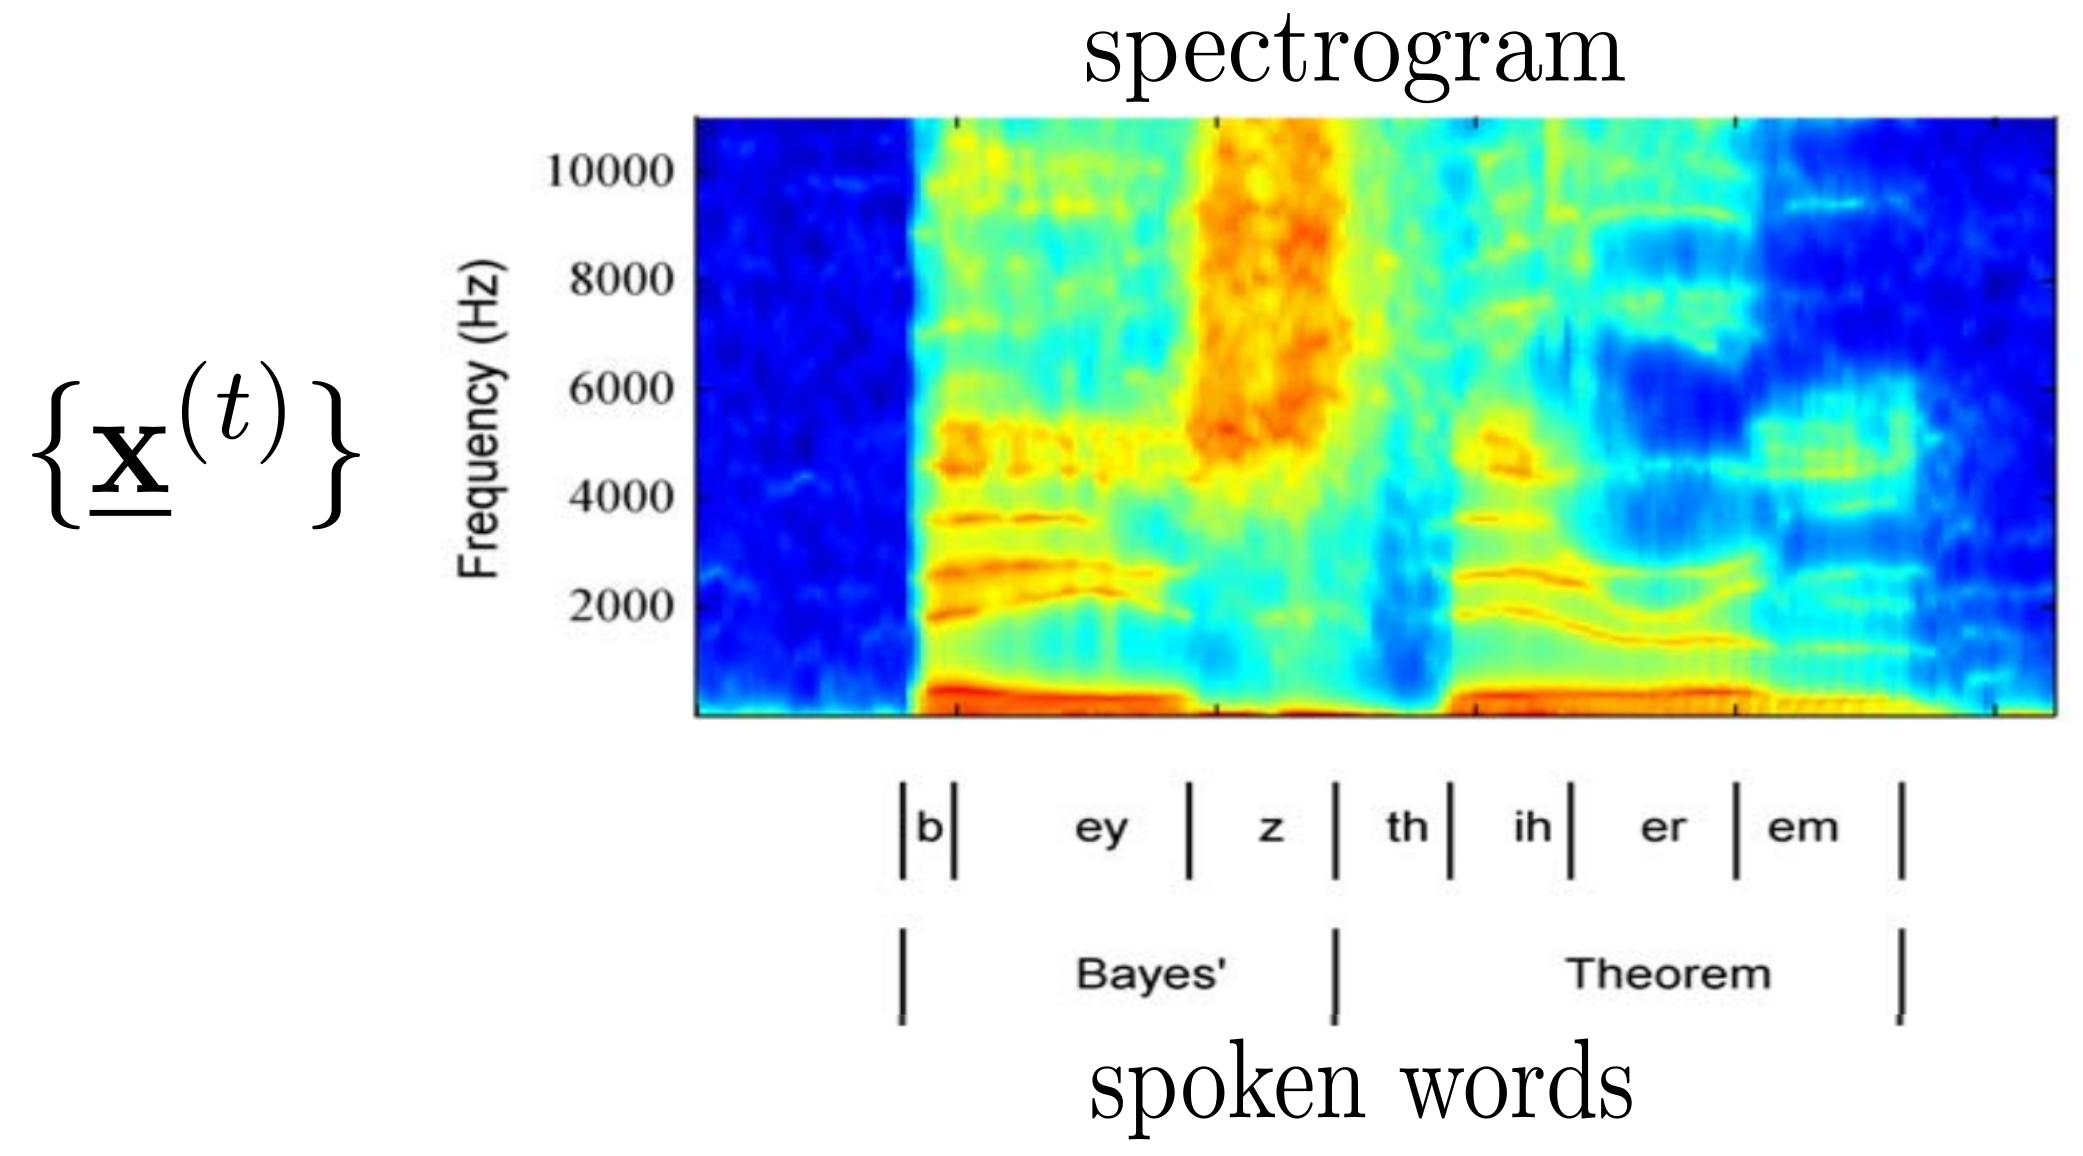
\includegraphics[width=0.6\textwidth]{img/Bishop_13-1}
	\slidesonly{\captionof*{figure}{Source: \citep{bishop2006pattern}}}
	\notesonly{\captionof{figure}{Source: \citep{bishop2006pattern}}}
\end{center}

\item<only@2> If we are interested in the \emph{most likely} sequence, we employ the \emph{Viterbi algorithm}
to find:
\begin{equation}
\{\vec m_*^{(t)} \} = 
\argmax_{\{\vec m^{(t)} \}} P(\{\vec m^{(t)} \} | \{\vec x^{(t)}\} )
\end{equation}

\item<only@3>
If the dimensionality of $\vec m$ is much lower than $\vec x$ (e.g. 2-D vs. $N$-dim), we can sample from the posterior to visualize the sequence.

\end{itemize}

\end{frame}

\subsubsection{One-step-ahead prediction}

\begin{frame}{\subsecname:~\subsubsecname}

One-step-ahead prediction involves the conditional distribution:
\begin{align}
P(&\vec{x}^{(t+1)} ~|~ \vec{x}^{(1)}, \ldots, \vec{x}^{(t)}) 
= \\
&\sum_{\{\vec{m}^{(t+1)}, \vec{m}^{(t)} \}} P(\vec{x}^{(t+1)} | \vec{m}^{(t+1)}) \cdot P(\vec{m}^{(t+1)} | \vec{m}^{(t)}) \cdot~{\only<2>{\color{blue}}P(\vec{m}^{(t)} | \vec{x}^{(1)}, \ldots, \vec{x}^{(t)})}\\
\only<2>{
=& 
\sum_{\{\vec{m}^{(t+1)}, \vec{m}^{(t)} \}} 
\kern-2ex
P_{\mathit{emission}} \cdot P_{\mathit{tansition}} \cdot~{\color{blue}P(\mathit{the ~state~we~have~reached~so~far})}
}
\end{align}

\pause 

This only involves ${\color{blue}
P(\vec m^{(t)}, \vec x^{(1)}, \ldots, \vec x^{(t)}) 
}$ from the forward pass in addition to summing over the possible combinations of $\vec m^{(t)}$ and $\vec m^{(t+1)}$

\end{frame}
